Through chapters~\ref{chap:low_level} and~\ref{chap:high_level}, we have shown
that our simulation method is flexible, as it models low-level properties of the
hardware, but still allows the simulation of full applications on top of
high-level APIs. This opens the door to many potential studies using our
simulator. In this chapter, we present some ongoing work and ideas. Some are
already implemented, but require additional work to be considered as fully
completed, while others are only ideas that can be explored in future work. In
particular, we will present a study on flow-control, which is a feature being
investigated as part of the design process for the next-generation BXI hardware.
We also present a few ideas of how S4BXI could be used in the future.

\section{Flow control in BXI}

In networking, flow-control consists in limiting the amount of data that can be
sent on a given channel, typically to avoid saturating a shared link. The
flow-control currently available in Portals only covers a very specific issue: a
``flow control situation'' happens when a node receiving messages runs out of
resources to handle the incoming traffic (for example when there is no ME or LE
to process a request). When this happens, the target NIC completely disables the
corresponding Portals Table entry (PT), which will cause the initiator NIC to
receive ACKs with an error status, and it notifies the user application. It is
then the responsibility of the application to fix the problem which triggered
flow-control, and enable the PT again. This mechanism is designed to handle
extreme cases of resource exhaustion, and leaves a lot of responsibility to the
application. The hypothesis we want to test is whether it would be beneficial to
implement a different version of flow control, where the NICs would limit the
number of messages inflight to another node, which would lower the congestion on
the cluster, and avoid situations of resource exhaustion. In particular, we want
to test two cases: limiting the number of messages inflight between two NICs,
and limiting the number of messages inflight between two processes. As it turns
out, these two options are already implemented in software in OpenMPI.
Therefore, it would be interesting to compare the performance of the network
when this type of flow control is enabled in software, in OpenMPI, and when it
is implemented in hardware directly. To test this last scenario, a real-life
experiment would require the design and manufacturing of several NICs, while we
can estimate the effect of this change with a few modifications of our
simulator.

\begin{figure}[!ht]
    \centering
    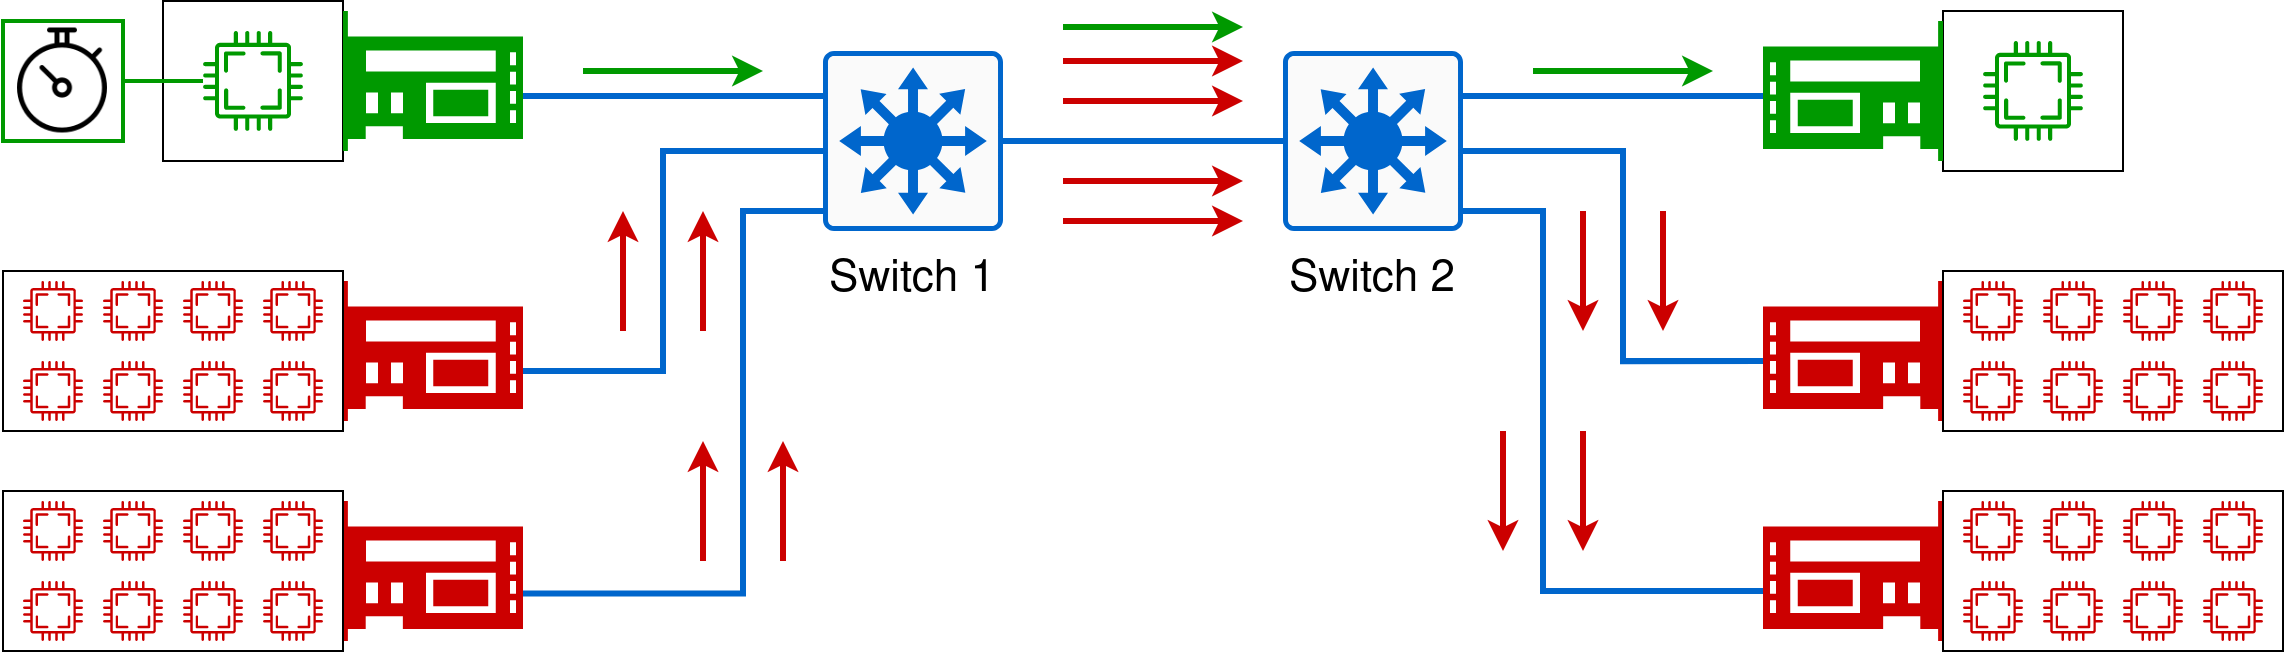
\includegraphics[width=1\textwidth]{7_flow_control/experiment.png}
    \caption{Our flow control experiment}
    \label{fig:7_flow_control:experiment}
\end{figure}

In order to check the efficiency of the different flow control implementations,
we designed the experiment depicted on
Figure~\ref{fig:7_flow_control:experiment}: our simulated platform consists of
two switches connected together, with the same number of machines connected to
each switch. This way machines connected to \textit{Switch 1} that communicate
with machines connected to \textit{Switch 2} will share a common BXI Link. While
this is a very simple topology, it is representative of real-world scenarios as
pruning is very common in HPC clusters, which means that most of the time there
will be shared links of this sort between switches (this is especially common in
fat-tree topologies). The workload that we simulate is simple: pairs of machines
(two in the figure) run several processes each (eight in the figure), which will
flood the network by sending as many 16MB messages as possible to each other.
While this is not what a realistic application would do, it does emulate
realistic situations where an application running on many nodes would have an
intense communication phase. On the other hand, the remaining pair of machines
simply runs one process each, which sends a fixed amount of 16MB messages
sequentially. We measure the latency between the second pair of machines (top
pair of Figure~\ref{fig:7_flow_control:experiment}), which gives us an estimate
of the congestion on the shared BXI link.

\begin{figure}[!ht]
    \centering
    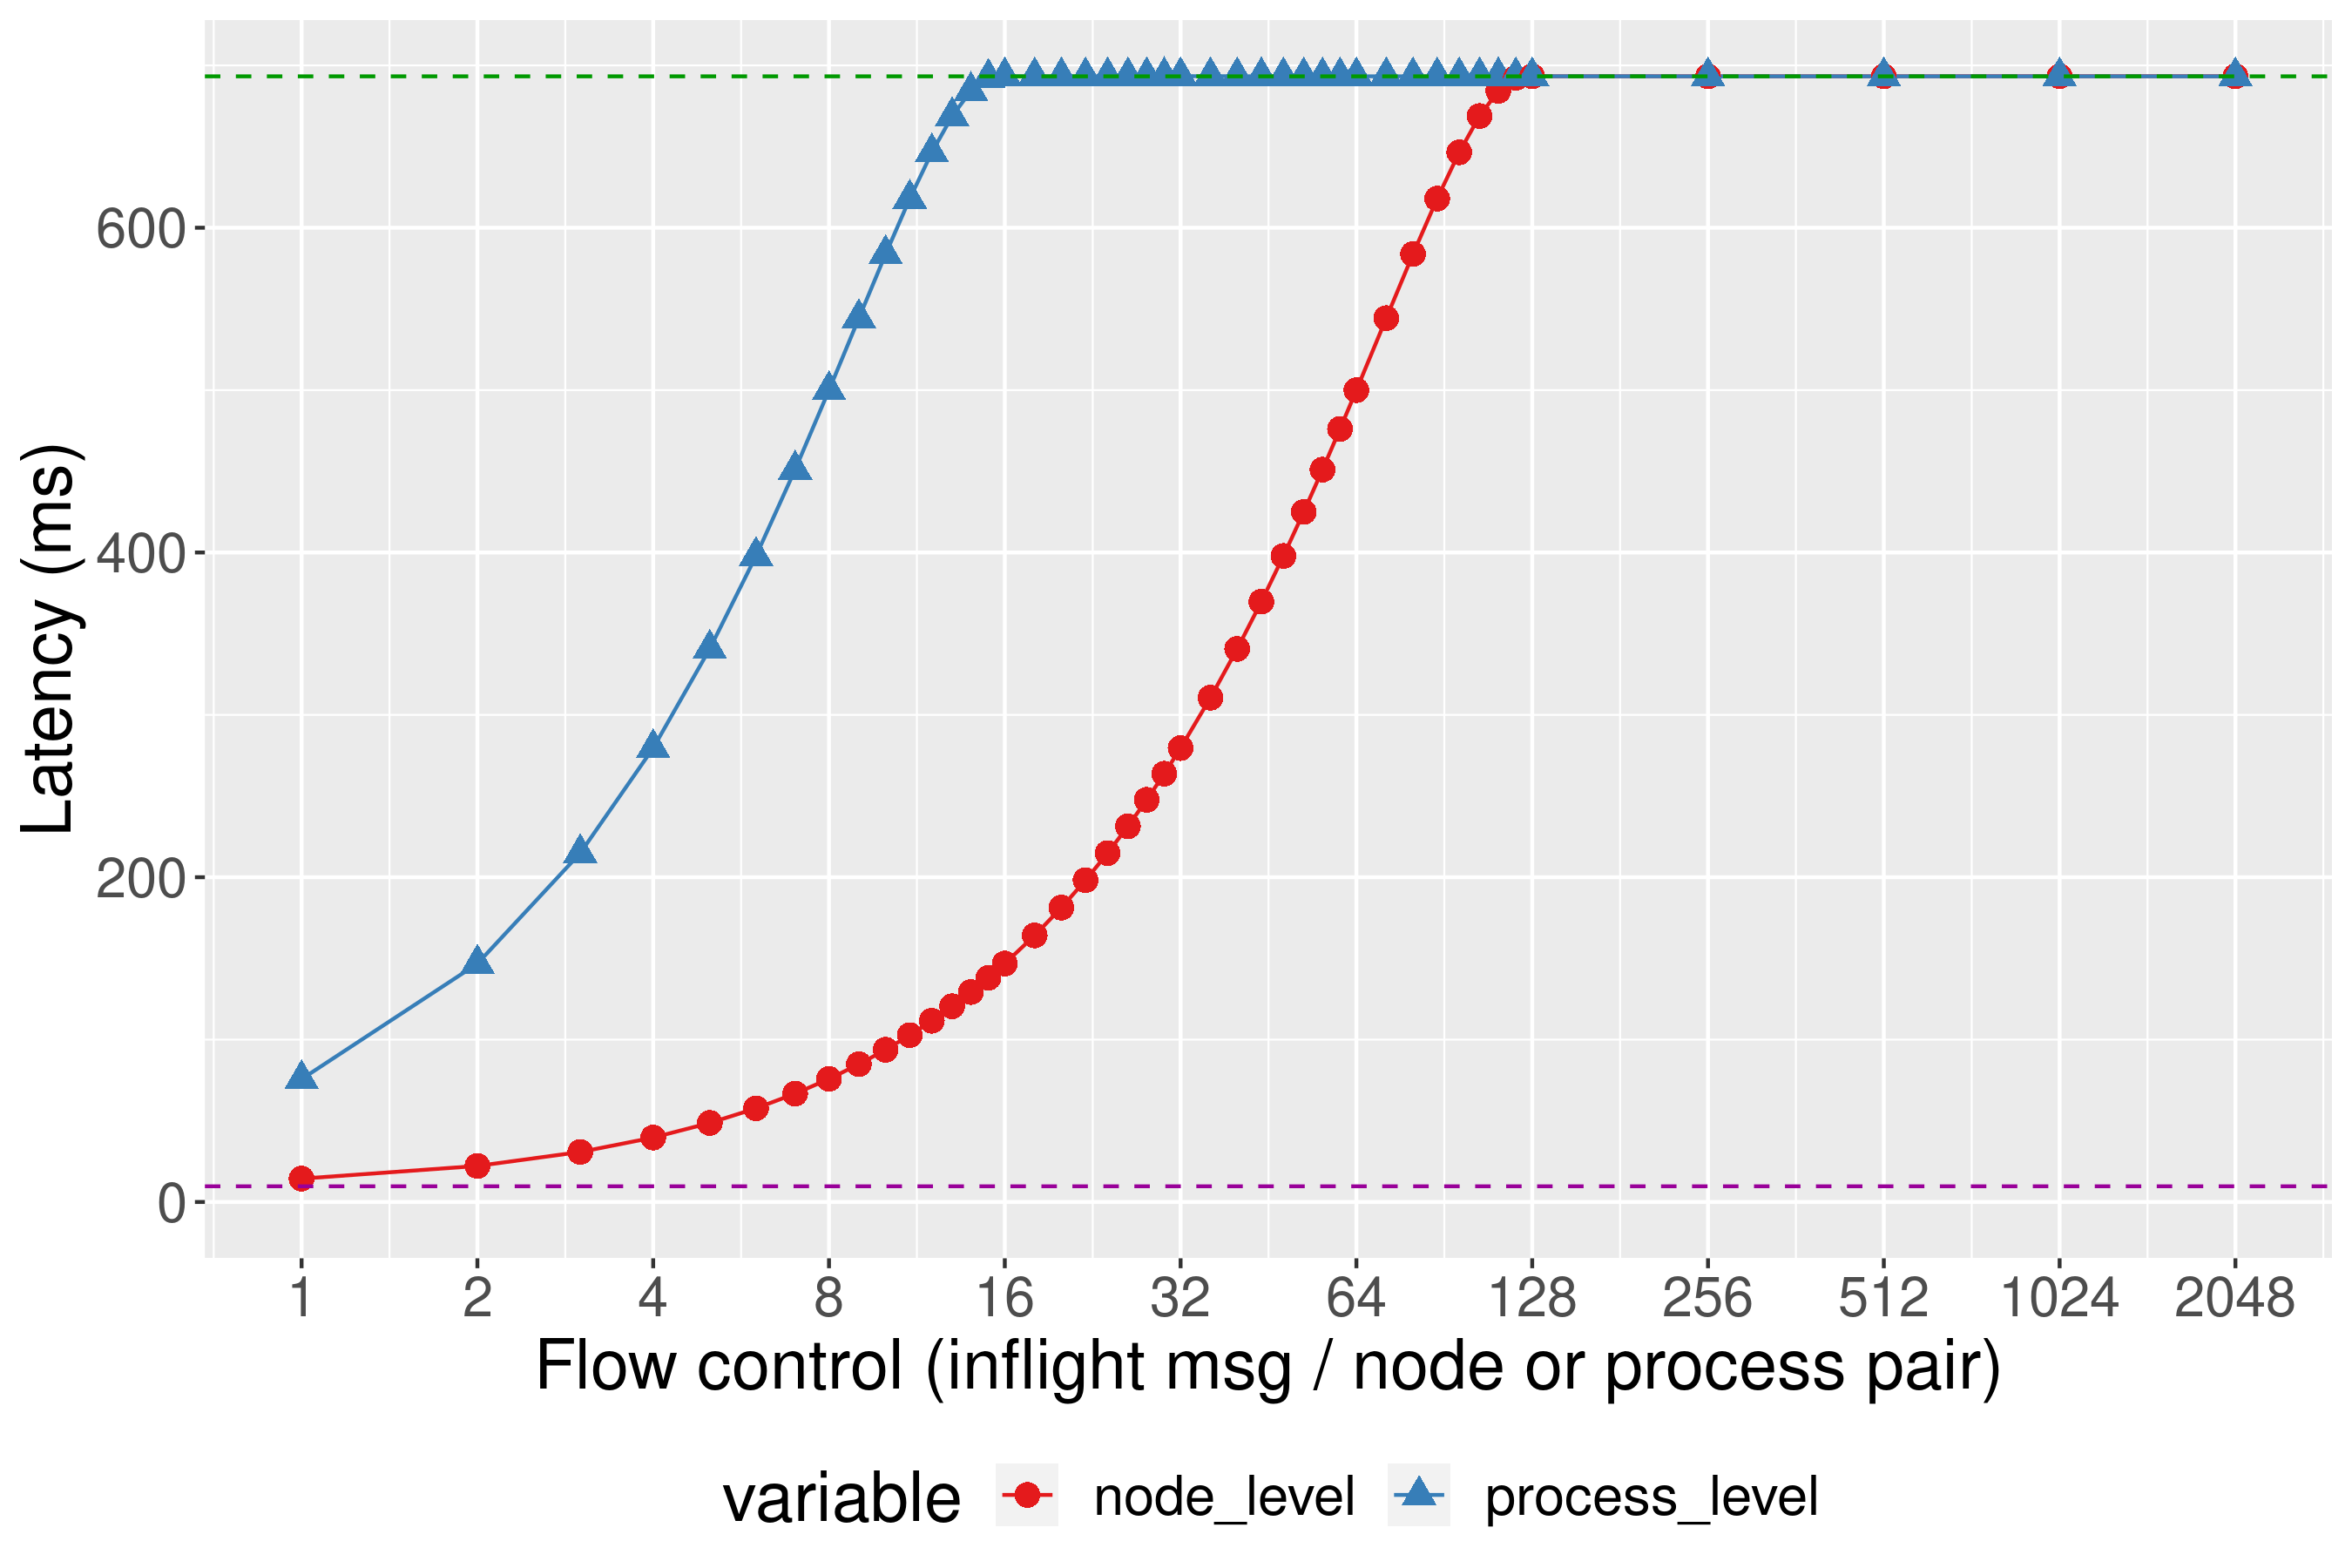
\includegraphics[width=1\textwidth]{7_flow_control/1M_full_portals_8ppn_1floodPair.png}
    \caption{Results of our flow control experiment with Portals, 1MB messages, 1 pair of nodes flooding the network with 8 processes per node}
    \label{fig:7_flow_control:1M_full_portals_8ppn_1floodPair}
\end{figure}

As this experiment was conducted in parallel with the rest of our work (in
particular in parallel with the simulation of MPI), it evolved along with our
simulation method. Initially, we implemented this small benchmark with Portals
directly, and measured the latency of sequential messages for different values
for our flow control: how many messages are allowed inflight between pairs of
nodes or pairs of processes. The result of our simulations at that time is
depicted on Figure~\ref{fig:7_flow_control:1M_full_portals_8ppn_1floodPair},
which was obtained for messages of one megabyte and only one pair of machines
flooding the network (with eight processes on each machine). On this figure, the
lowest horizontal line corresponds to the latency of messages when no machine is
flooding the network (which correspond to a simple point-to-point sequential
transfer). The top dotted line corresponds to the latency of sequential messages
when flooding machines are at their full speed, with no flow control at all
(which is what the current BXI hardware would do). The two curves correspond to
the latency of messages for different values of process-level flow control, and
node-level flow control. The two curves are very similar except one is a
translation of a factor eight along the x-axis of the other one; this is
expected since flooding machines run eight processes each, therefore node-level
flow-control is roughly eight times stricter than process-level flow-control. We
can also see that if we limit the number of messages inflight to the extreme,
the latency of messages gets very close to the scenario when no one is flooding
the network. Even though our experiment is quite artificial, it gives us an idea
of the effect that flow-control implemented in BXI hardware could have on the
congestion on a cluster.

\begin{figure}[!ht]
    \centering
    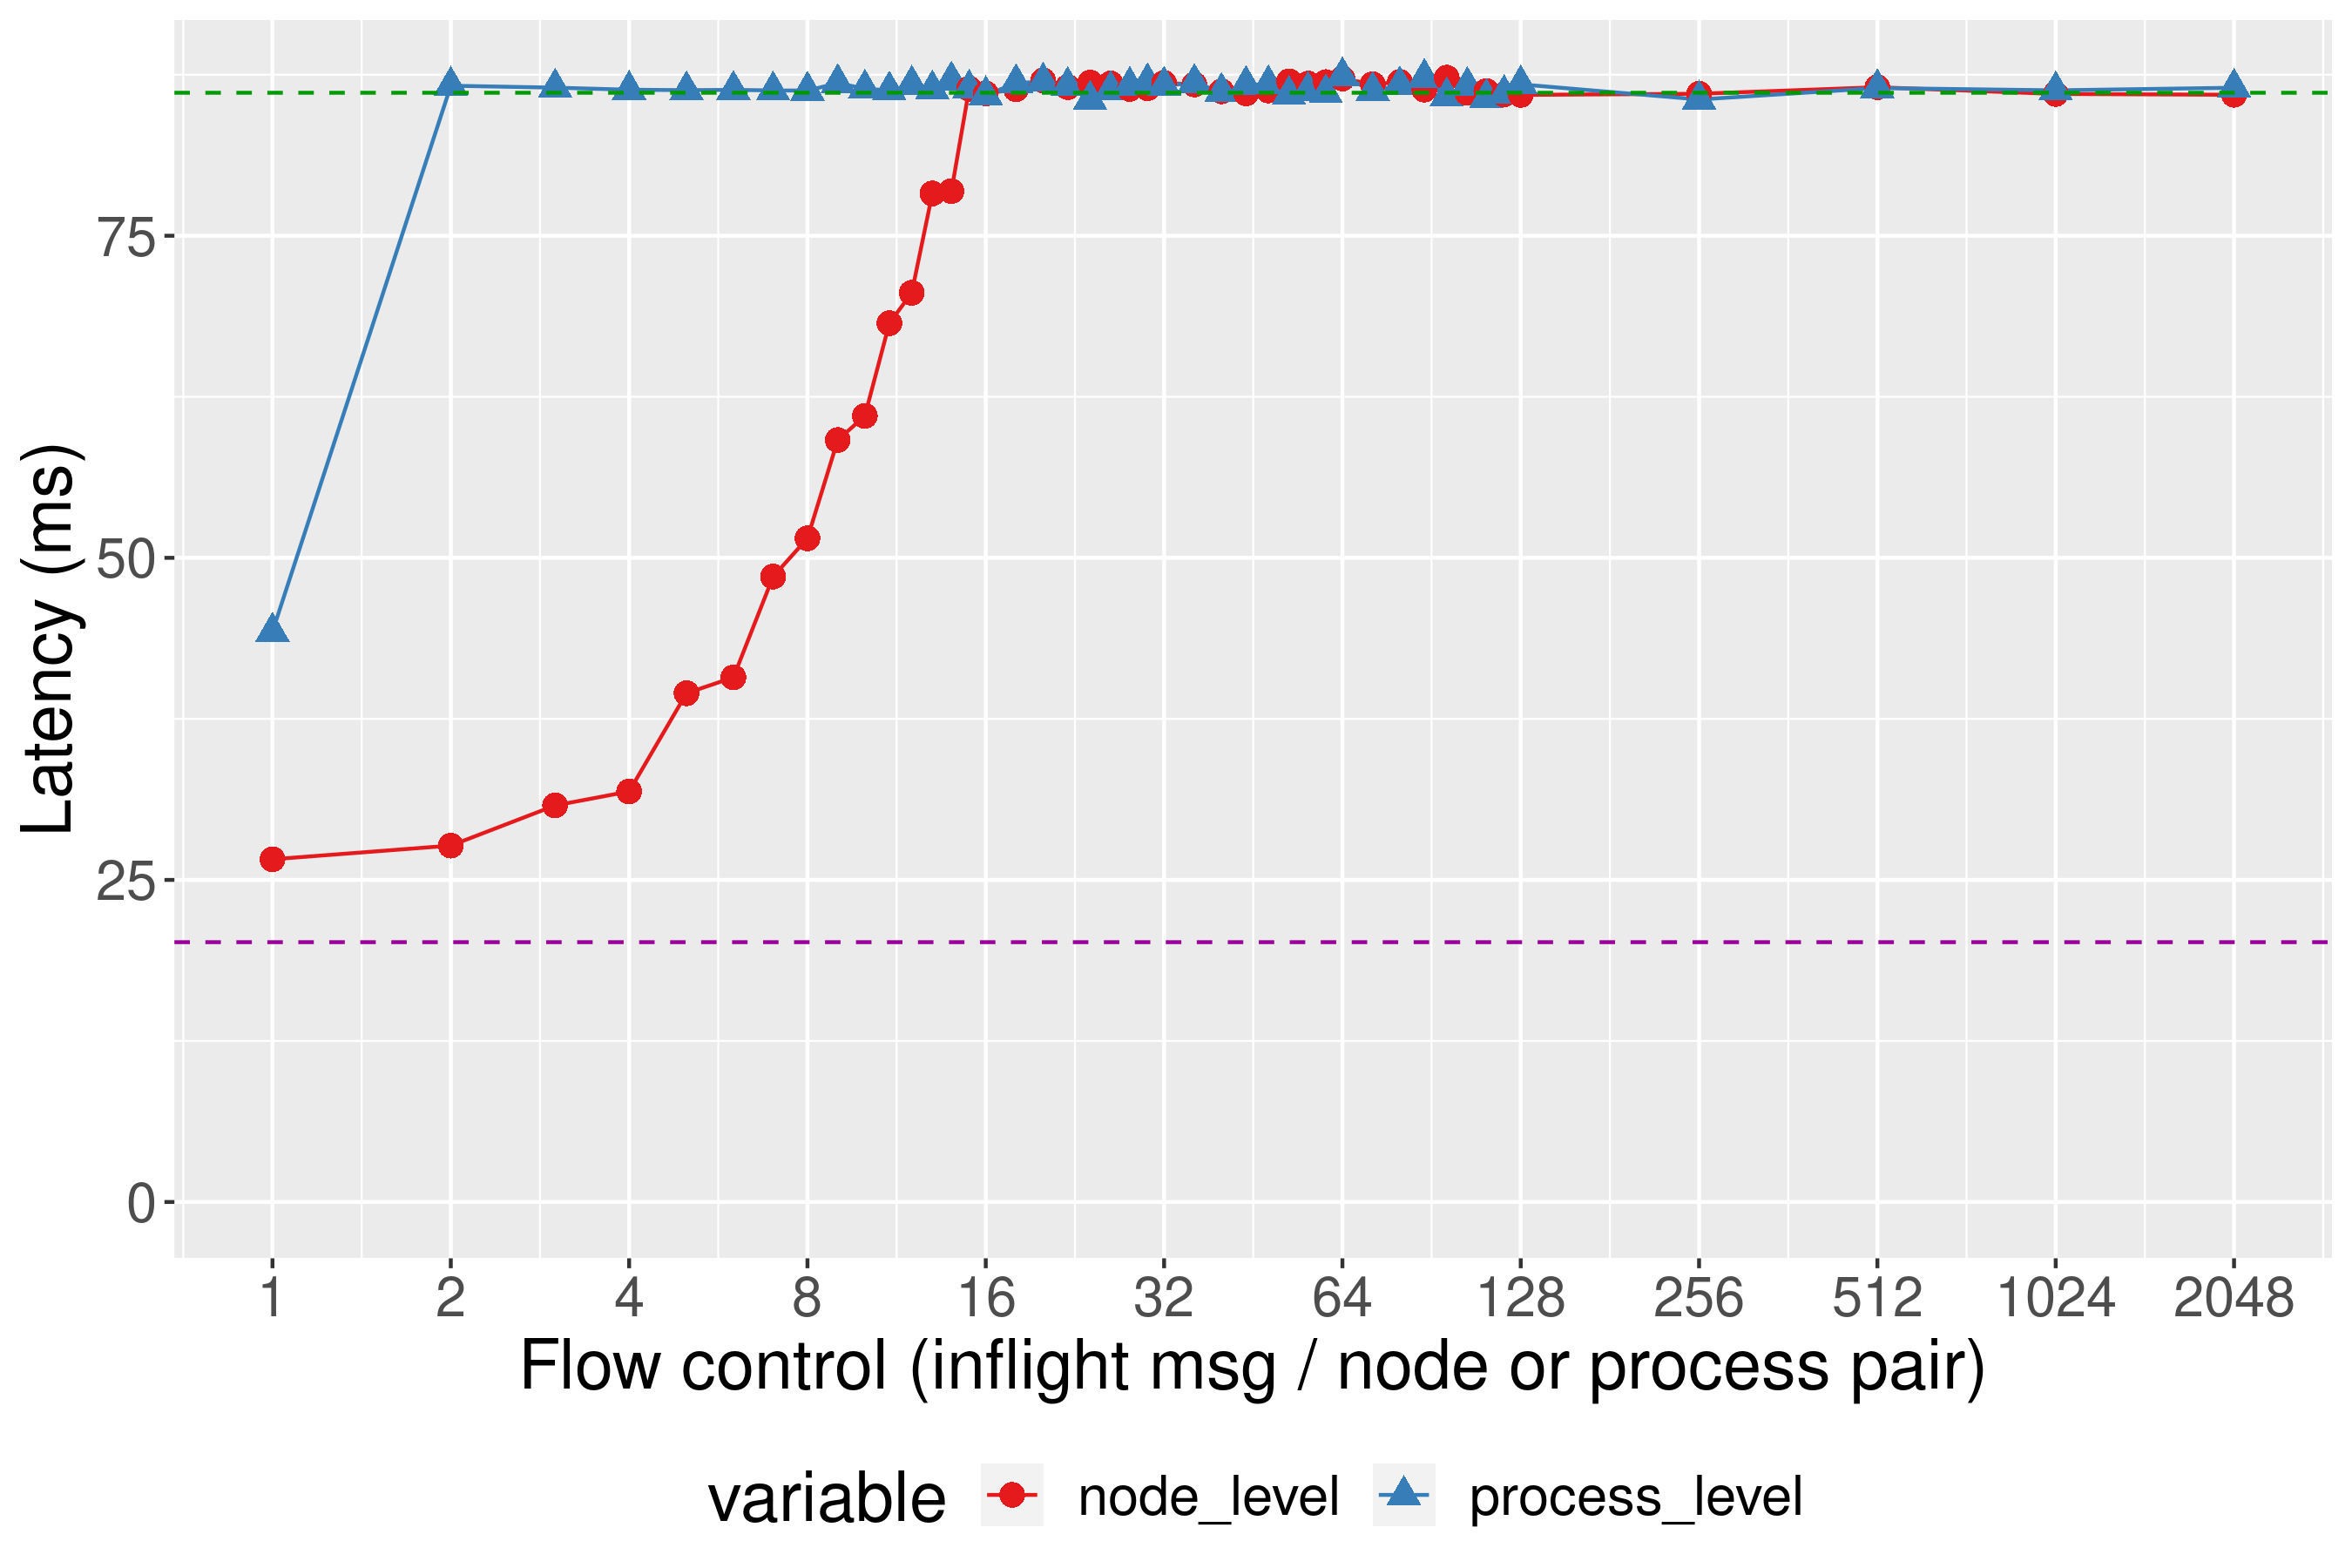
\includegraphics[width=1\textwidth]{7_flow_control/1M_full_MPI_8ppn_1floodPair.png}
    \caption{Results of our flow control experiment with MPI, 1MB messages, 1 pair of nodes flooding the network with 8 processes per node}
    \label{fig:7_flow_control:1M_full_MPI_8ppn_1floodPair}
\end{figure}

As we progressed in our work, we did our flow-control experiment again, but in
more realistic conditions, using MPI instead of Portals. Therefore, we
re-implemented our benchmark, as close as possible to the original one, but
using OpenMPI instead of directly Portals for our communications. Running the
experiment in the same conditions as previously gave us the results depicted on
Figure~\ref{fig:7_flow_control:1M_full_MPI_8ppn_1floodPair}. We can see that
even though flow-control still affects the congestion on the network, the
difference between a strict flow-control and no flow-control at all is much
smaller. From this experiment, it seems that when messages are not slowed down
by congestion, they can go nearly as fast with MPI as they were going with
Portals directly. On the other hand, when we try to add congestion to the
network, the nodes flooding the network do not manage to send as many messages
inflight as previously. Therefore, the sequential transfers that we measure are
not slowed down as much, and flow-control does not have an impact as important
as previously. The conclusion we can draw from this experiment is that even
though flow-control seems like an interesting feature to have in theory, in a
real-world scenario there are many factors which can affect the amount of
congestion on the network, which is why this type of simulation is a good tool
to measure the expected performance of this type of feature.

\begin{figure}[!ht]
    \centering
    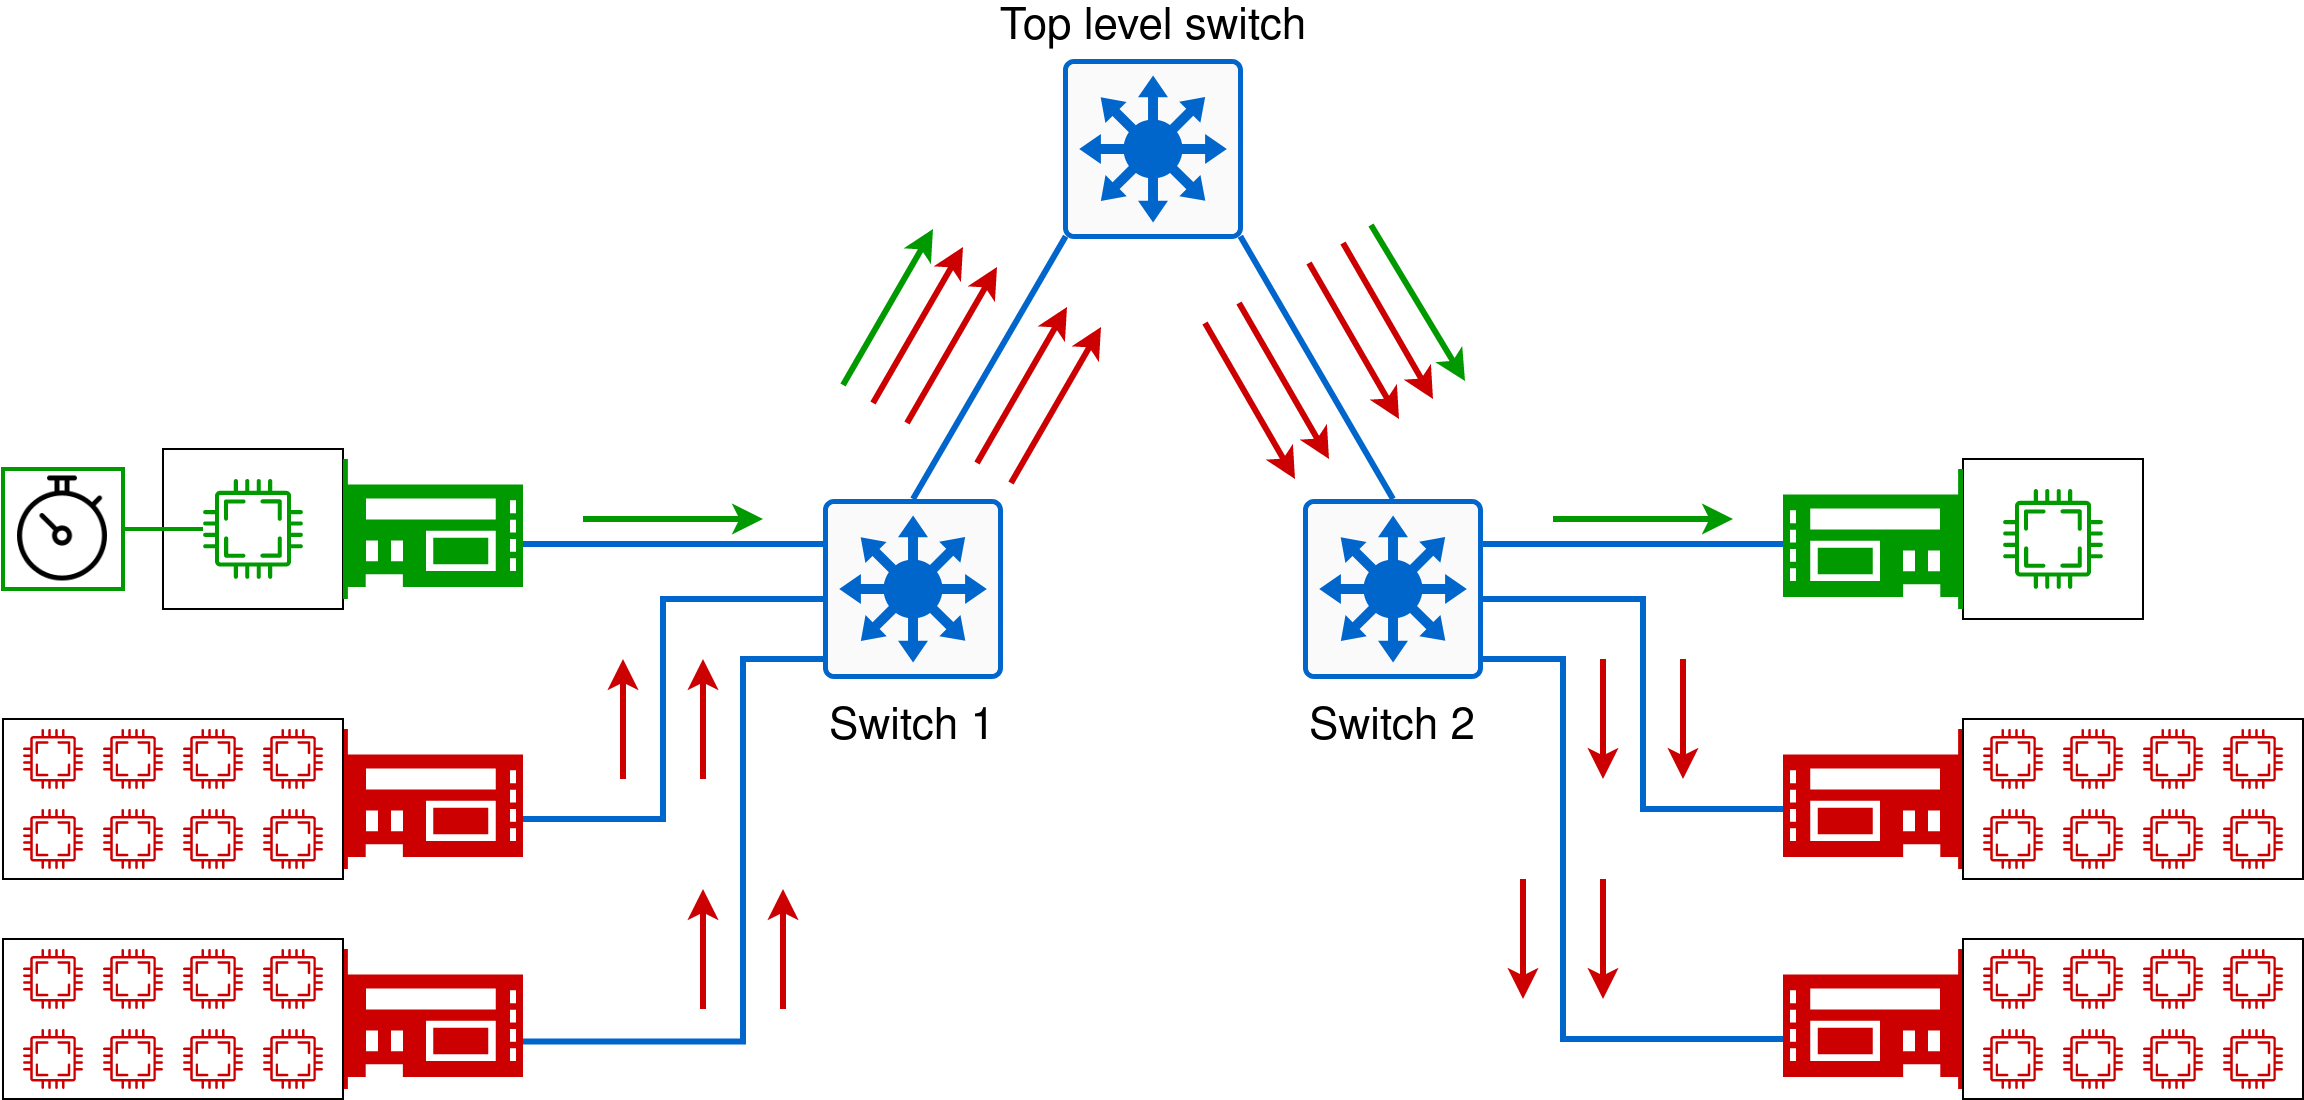
\includegraphics[width=1\textwidth]{7_flow_control/vix.png}
    \caption{Flow control experiment compatible with our real-world cluster}
    \label{fig:7_flow_control:experiment_vix}
\end{figure}

Finally, we tried re-creating our experiment in a setting that is comparable
with a real-world experiment, in order to increase our confidence in our
simulation results. Of course, it is impossible to re-create our experiments on
a real-world cluster, since the flow-control that we propose is not implemented
in BXI v2 hardware. What we can compare in simulation and in the real world,
however, is flow-control implemented in software. In particular, Atos's version
of OpenMPI offers two parameters to control the number of messages inflight in
the BXI BTL: one to configure the limit of messages inflight, and one to control
whether the ``inflight message counter'' should be shared between all processes
of a node or not. By combining these two options, we can emulate in software an
experiment which is quite close to the scenarios that we explored in simulation
previously. Unfortunately, we realized that running the real-world experiment
would also require changing our cluster's topology slightly: indeed, we did not
have any machines available which were connected in the configuration depicted
on Figure~\ref{fig:7_flow_control:experiment} (as it is very rare to have to
switches connected to compute nodes and also directly together). Indeed, while
this type of platform exists in Torus networks, in BXI we only have access to
fat trees, where switches with compute nodes are not directly connected to each
other, but instead they are connected to a higher level of switches (closer to
the root of the fat tree). Therefore, we changed our experiment slightly, to the
configuration depicted on Figure~\ref{fig:7_flow_control:experiment_vix}. 

\begin{figure}[!ht]
    \centering
    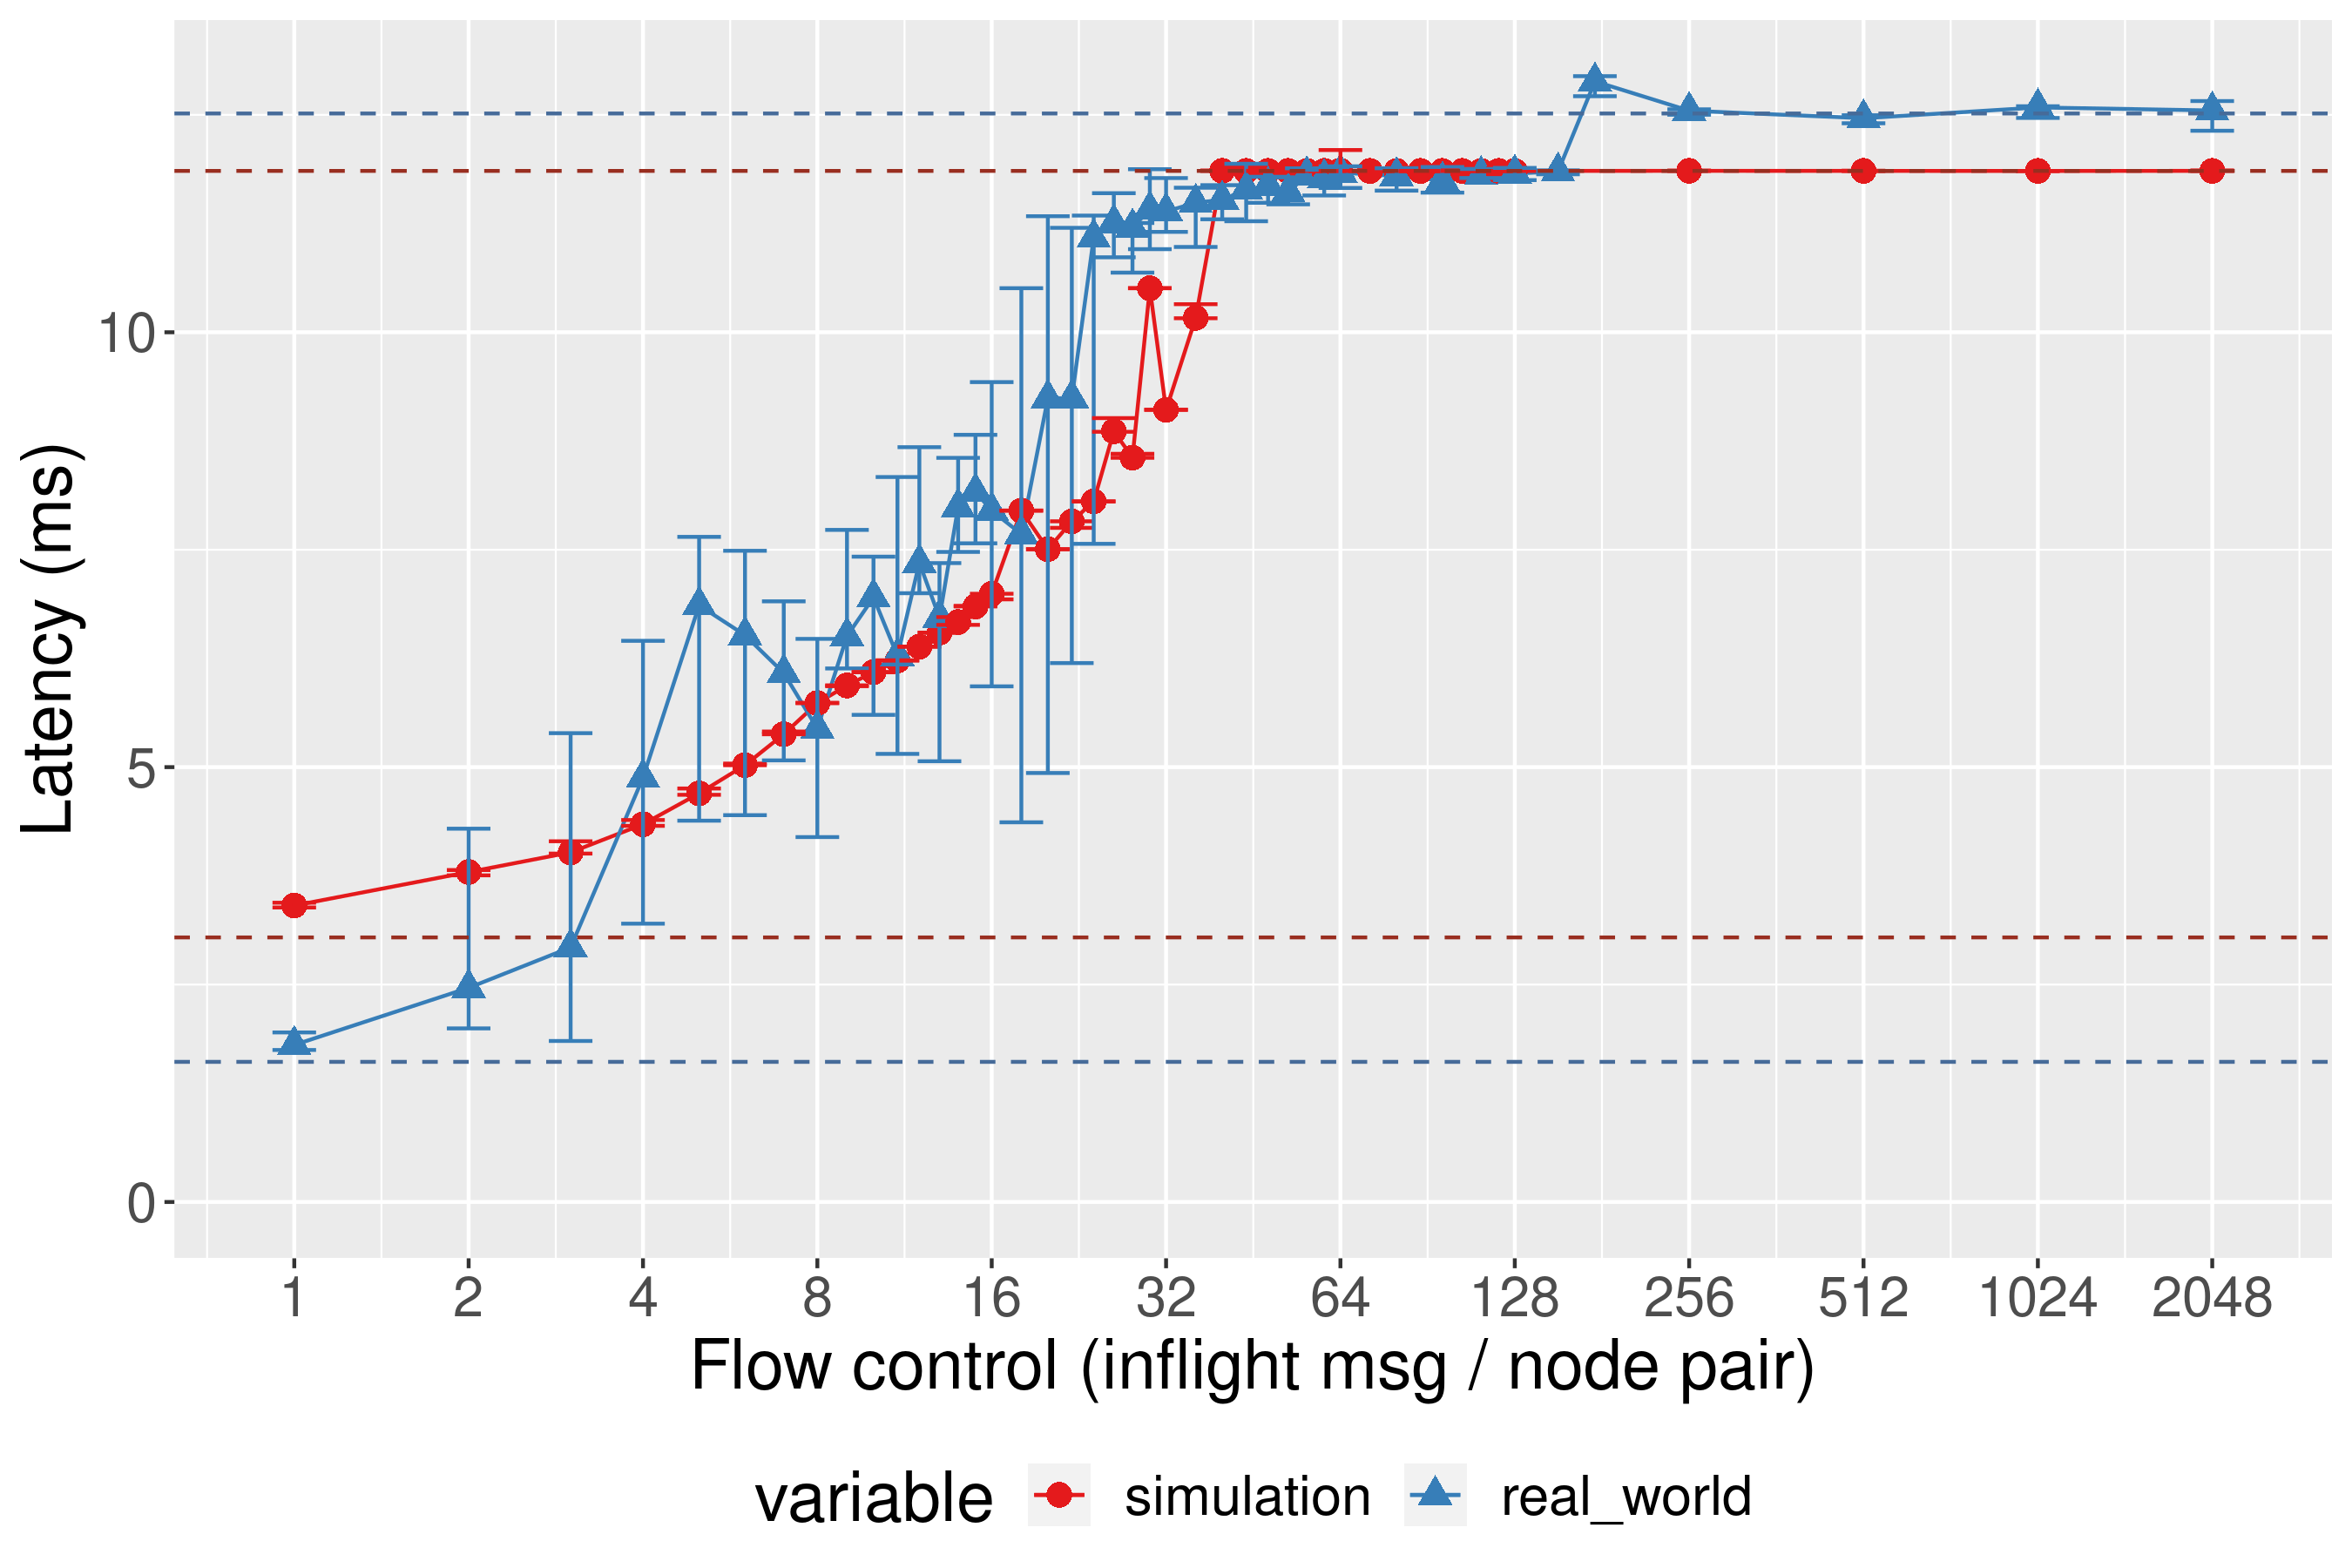
\includegraphics[width=1\textwidth]{7_flow_control/16M_compare_node_level_real.png}
    \caption{Node-level software flow control in OpenMPI, 16MB messages, 4 pairs of nodes flooding the network with 8 processes per node}
    \label{fig:7_flow_control:16M_compare_node_level_real}
\end{figure}

\begin{figure}[!ht]
    \centering
    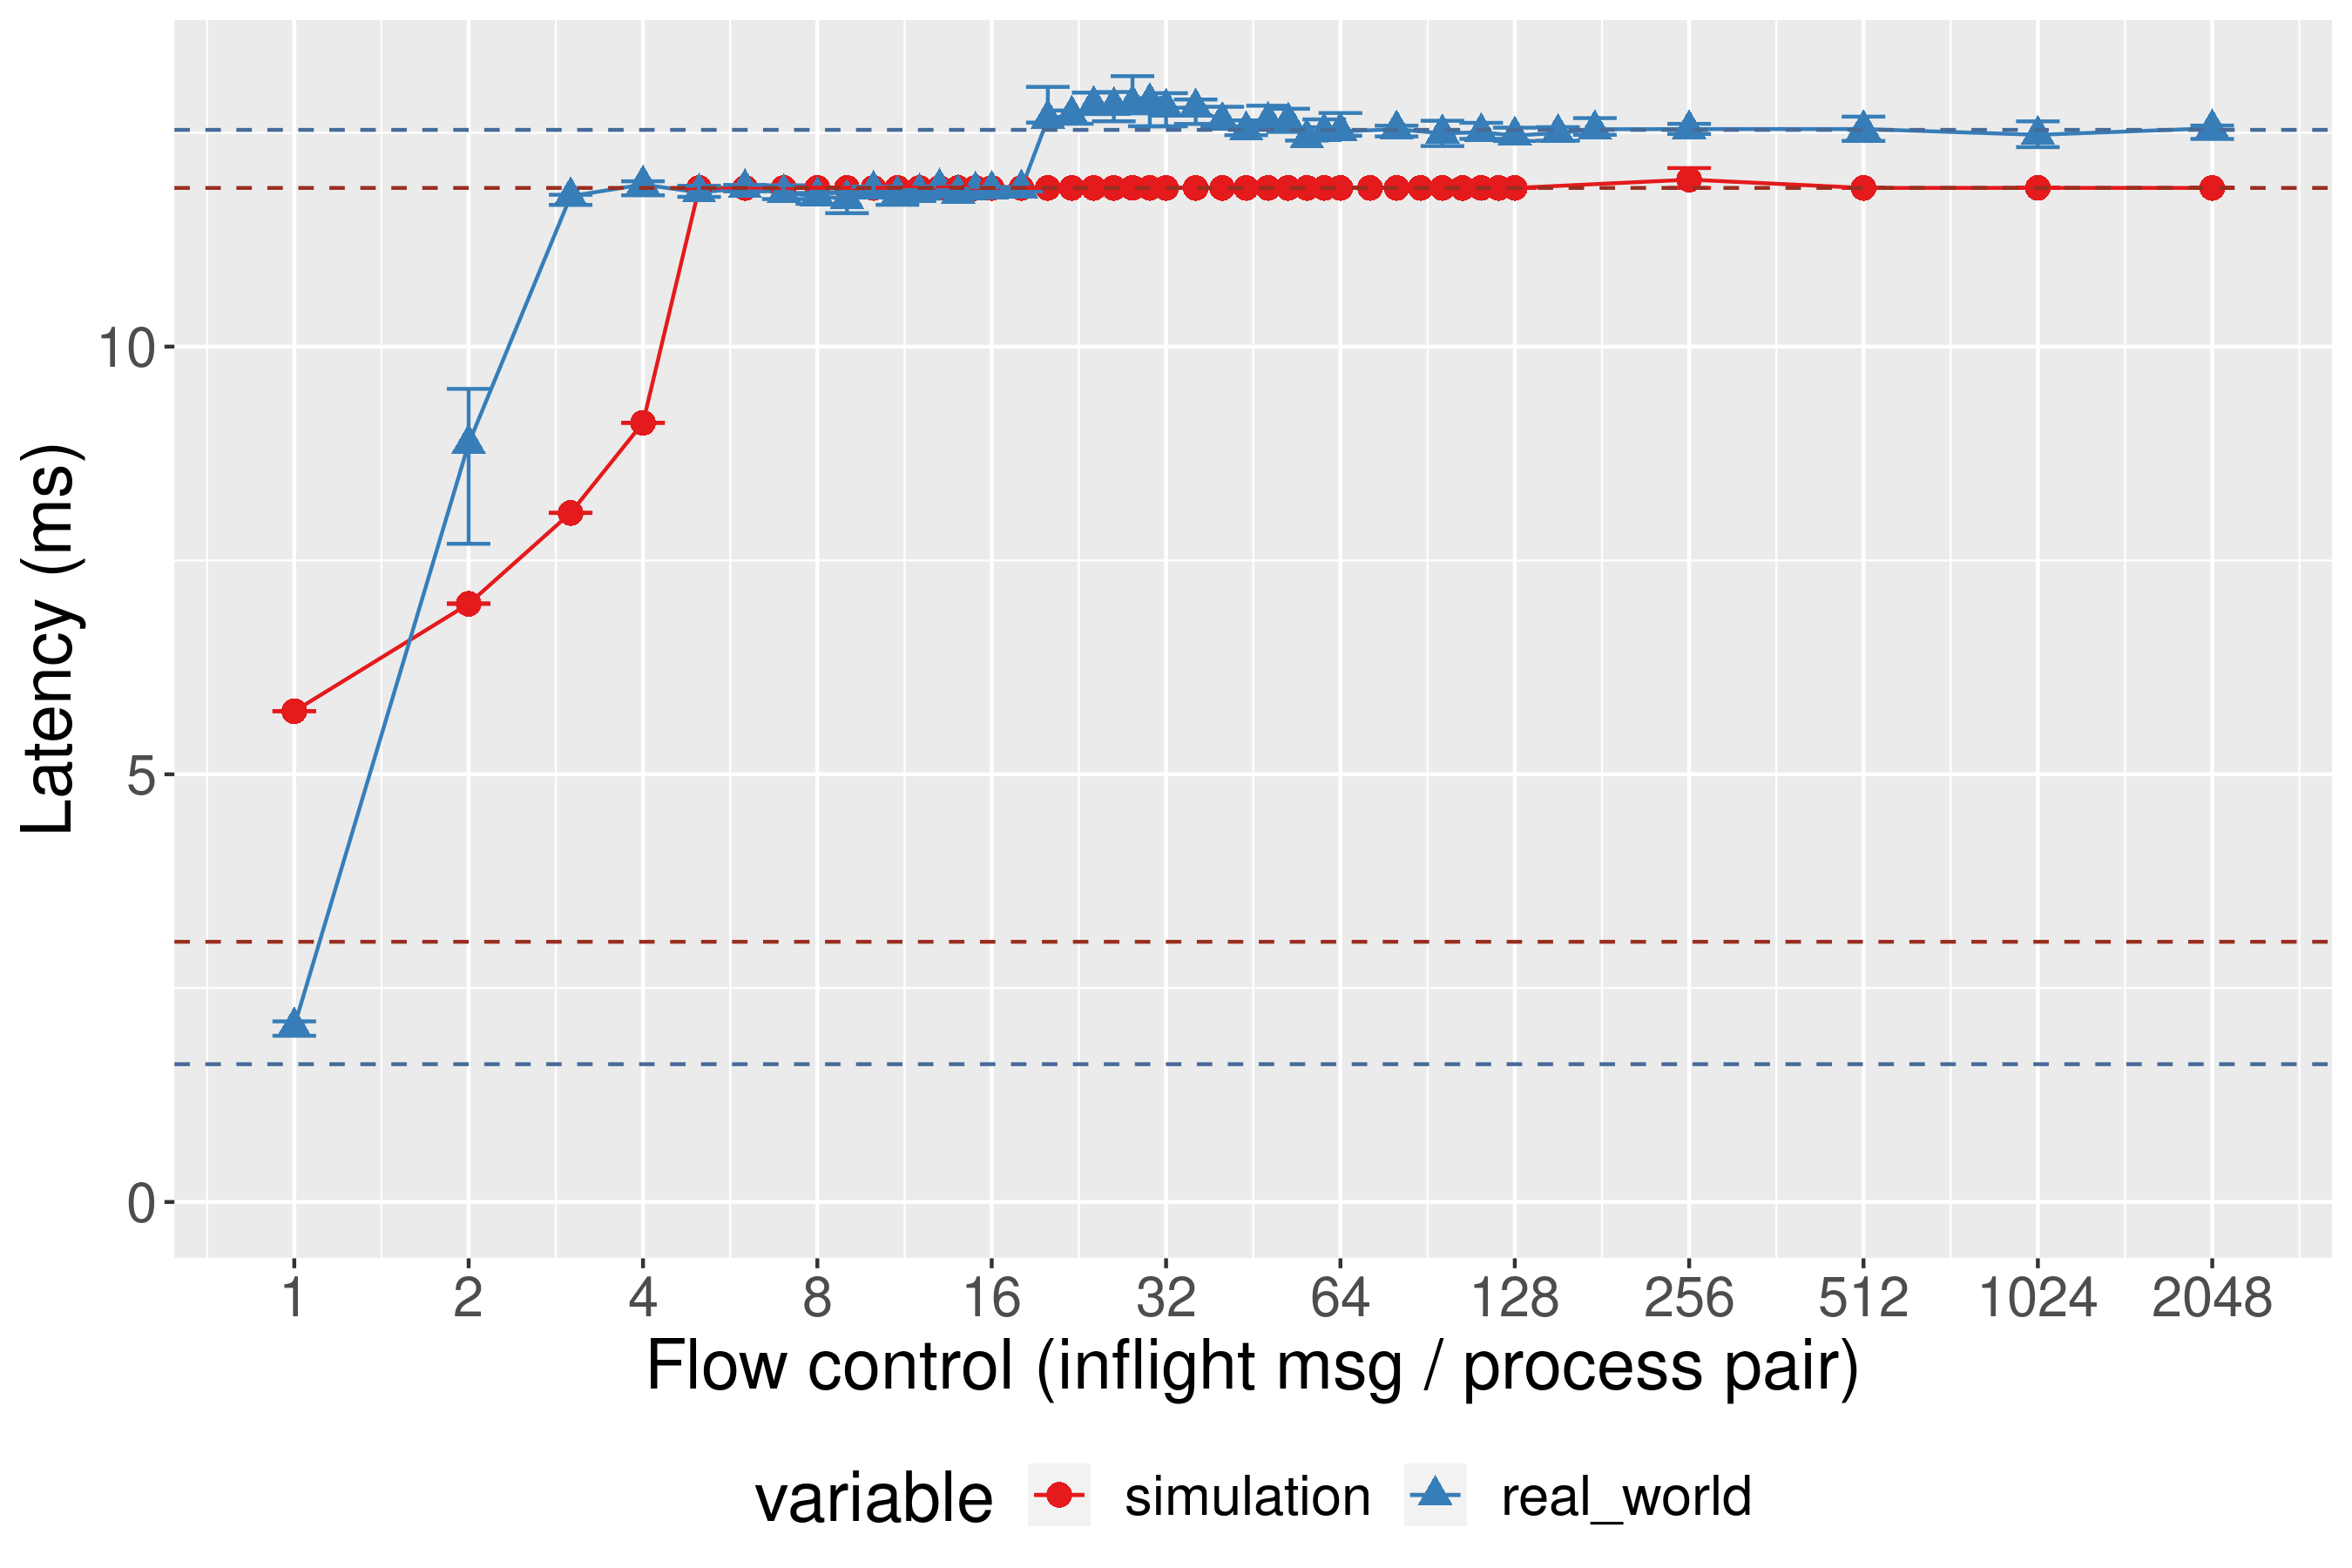
\includegraphics[width=1\textwidth]{7_flow_control/16M_compare_process_level_real.png}
    \caption{Process-level software flow control in OpenMPI, 16MB messages, 4 pairs of nodes flooding the network with 8 processes per node}
    \label{fig:7_flow_control:16M_compare_process_level_real}
\end{figure}

For this experiment, both the simulation and the real-world cluster use the
software flow-control implemented in MPI. The results are displayed on
Figure~\ref{fig:7_flow_control:16M_compare_node_level_real} for node-level
flow-control, and on
Figure~\ref{fig:7_flow_control:16M_compare_process_level_real} for process-level
flow-control.

It is important to note that in this configuration, we had difficulties
obtaining meaningful results on the real-world cluster for two reasons. First,
the machines used were quite slow, and we did not manage to create any
significant congestion on the network, therefore we had to increase the message
size to 16 megabytes, and to use four pairs of machines flooding the network
(instead of just one previously). Second, we observed a lot of variations in our
data, which made it very difficult to analyze. In an attempt to improve this
point, we ran each real-world experiment ten times, and we removed the two
biggest and two smallest values for each point, as we often saw ``extreme''
data-points with unrealistic values, which we believe must have been affected by
phenomenons outside of our control. 

Regardless, we can see on both figures that even though our simulator is far
from perfect, it captures well the order of magnitude that we can expect for the
latency of messages when software flow-control varies. This is especially true
for node-level flow-control (on
Figure~\ref{fig:7_flow_control:16M_compare_node_level_real}), where our results
are close to the real-world data. For process-level flow-control, we can see on
Figure~\ref{fig:7_flow_control:16M_compare_process_level_real} that setting the
limit of inflight messages to one gives an extremely short latency for the flow
of sequential messages, which we do not capture in simulation. Although this
behavior is unexpected from the real-world run, we can see that it is a lot more
consistent than other data points, as it has a very small variation across
several runs (depicted by the error bar). Another unexpected result that we can
see on both figures is the result for very lenient flow-control values: in both
cases we can see a ``jump'' in latency, around 16 messages inflight on
Figure~\ref{fig:7_flow_control:16M_compare_process_level_real} and around 128
messages inflight on
Figure~\ref{fig:7_flow_control:16M_compare_node_level_real}. Once again, this
behavior is unexpected from the real-world, as we do not believe that there
should be any special condition in OpenMPI's code to operate any differently
before or after this value. At a lower-level, in BXI, to the best of our
knowledge the only instance where this value could appear is in the size of the
command queues between the CPU and the NIC: each process can use 16 ``slots'' on
the NIC's memory to post commands. Therefore, it is possible that having to wait
for a free slot in Portals' library impacts the latency of flooder nodes
differently than restricting the number of messages inflight in OpenMPI, one
layer higher in the software stack. Unfortunately we lacked time to study
precisely these unexpected behaviors of real-world hardware, therefore we did
not test our hypotheses. Indeed, setting up experiments allowing us to validate
or not these experiments is not trivial.

\smallskip

To conclude, we can see that even though our model of congestion in the context
of software flow-control is not perfect, and does not take into account all the
properties of the real-world experiment, it still gives us a decent estimation
of the congestion that we can expect in such a scenario. These results give us
confidence that the data we obtained when modeling flow-control in hardware
shows the correct order of magnitude that we can expect for the congestion on a
cluster, if flow-control was implemented in hardware in the next-generation of
BXI NICs. Additionally, it is important to detail a few things about our
workflow during the writing of this PhD: for every single experiment (real-world
or simulation, S4BXI or SMPI) in
chapters~\ref{chap:low_level},~\ref{chap:high_level}
and~\ref{chap:model_change}, our figures depict data that was obtained in the
last weeks of this PhD, in parallel with the writing of this document, in order
to ensure that all our experiments where reproducible with the latest version of
OpenMPI, SimGrid, SMPI and S4BXI (no matter how old the original developments
were). However, because of a lack of time and because of technical difficulties,
we were not able to reproduce the results regarding flow control. Therefore, all
the data of this chapter has been obtained a few months earlier, using the
versions of SimGrid, OpenMPI and S4BXI available on 16\textsuperscript{th} March
2022.

\section{Future work}

In addition to flow control experiments, our simulator and methodology are
versatile enough to open the door to many potential studies. This section
presents a few ideas that we did not have time to conduct ourselves.

\bigskip

\textbf{OpenSHMEM:} even though our work on OpenSHMEM already gave us promising
results, our study using this API is very preliminary. Indeed, in order to make
this type of simulation more robust, some bugs need to be fixed, and some
function calls that are not currently supported by S4BXI need to be intercepted
(and reimplemented in simulation), such as a few \inline{pthread} utilities
(mutexes for example, which would be easy to implement using SimGrid's Mutexes).
This would allow the simulation of larger scale OpenSHMEM applications, such as
the ``OpenSHMEM Benchmark suite'' (OSB)~\cite{OSB}. OpenSHMEM is a particularly
interesting API to study because it leverages the full capabilities of the
Portals API, whereas Atos's OpenMPI uses a more limited number of primitives
offered by Portals.

In order to improve OpenSHMEM support, a first idea would be to reference all
function calls that should be intercepted by our simulator, but are currently
not supported, to evaluate the difficulty of implementing them in simulation. It
would also be important to check the address of symbols that are located by
OpenSHMEM at startup, to see if the memory regions that are involved are
different on each simulated process or not. If the addresses are identical, a
modification to OpenSHMEM's initialization would probably be necessary to use
unique regions in each process, and better isolate them.

\bigskip

\textbf{Additional low-level studies:} it is important to note that even though
our simulator offers a fairly low-level model, it is not suited to study effects
that are visible at packet-level in the real-world. Nevertheless, our
flow-control experiments show that S4BXI can be used to study the protocol
implemented by BXI NICs in interesting ways. We believe that more experiments of
this type could be performed, to test the different ways that Portals can be
implemented.

As an example, the latest BXI hardware has a feature to disable end-to-end
reliability, which is also supported in S4BXI, but we do not believe that the
impact of this option on the performance of application has been studied in
great detail. In this context, S4BXI could be used to evaluate the implications
of making Portals unreliable, both in terms of functionality (how user
application could handle the loss of a message), and in terms of performance
(how big of a latency is saved by reducing the number of ACKs).

\bigskip

\textbf{Additional MPI studies:} one of the strengths of S4BXI is that it allows
users to replicate how the real-world Atos's MPI implementation works, in
particular regarding the algorithms used for collective operations. This means
that it would be a good tool to tune the collective algorithm to be used for
different message sizes and cluster sizes. Indeed, this precise tuning is
currently done on real machines, which is very time-consuming on a limited
amount of computing resources. In particular, it is very difficult to tune
operations for more than 32 nodes, as the development clusters at Atos are
small. This usage of the simulator has been discussed with the MPI development
team at Atos, but it has not been done yet, because we chose to focus on the
simulation of larger scale application. Nevertheless, tuning this type of
algorithms would be a very good use case of S4BXI, as we have already seen in
our benchmark that our approach models this selection accurately.

\bigskip

\textbf{Further Vader tuning:} currently all operations regarding shared memory
in MPI (using the Vader BTL) are considered as ``CPU time'' by S4BXI, as all of
MPI is considered as ``user code'' from the point of view of our low-level
model. This means that copies of data in memory are simply benchmarked and then
injected in the simulated time, similarly to how all computation time is
accounted for. We believe that it would be more accurate to stop the benchmark
of CPU time when entering the Vader BTL, and inject a set amount of time, that
would be carefully calibrated as a function of the size of data to be
transferred between MPI ranks. Indeed, the performance of memory accesses might
exhibit a different performance when simulated processes run one at a time (in
our single-threaded simulator), or all in parallel (in a real-world execution),
therefore modeling these operations using a well-calibrated model could give
better results. This approach would require patching OpenMPI further, and
designing a way to calibrate the time that Vader operations take, but we believe
that it would make the simulations more reproducible, as it would reduce the
amount of benchmarked CPU time. This work would be very similar to the study
that Tom \textsc{Cornebize} conducted on HPL by benchmarking the
\inline{HPL_dgemm} function, therefore an efficient methodology to conduct this
type of study is already available.

\bigskip

\textbf{Perturbations on the network:} in the simulated world, communications
always complete gracefully, with no error. However, we know that in the real
world a cluster can suffer from perturbations, for example data corruption
(detected at the target side by a CRC check), or transient failures of some
cables. In these cases, it is the responsibility of the E2E component of the NIC
to retransmit messages, which has a huge impact on performance. These types of
issues were not studied in depth in S4BXI, but it would be a good use case of
our simulator. Indeed, S4BXI fully implements the E2E reliability of BXI, and
SimGrid provides options to specify a ``profile'' for each Link, in order to
disable it at specific times in the simulation. Such experiments could help
improve the configuration of the E2E component of BXI, in particular the delay
used before retransmitting messages.

\bigskip

\textbf{Support for a wider range of parallelization techniques:} currently
S4BXI only supports Portals, MPI and to a degree OpenSHMEM, although in a
realistic scenario many applications support running computations in parallel
using both MPI and OpenMP. Currently, any OpenMP primitive would not be
intercepted in S4BXI (or SMPI for that matters), and therefore it would spawn
actual threads in our otherwise single-threaded simulation. As long as parallel
sections in OpenMP do not perform any network operation (or any operation that
could yield to SimGrid's scheduler), the application should run properly, and
probably give a result that is close to what the user expects. However, this
methodology is very fragile: it would be much safer to find a way to intercept
the creation of threads by OpenMP, and reimplement them in simulation using
SimGrid Actors. This study is very ambitious, as it would probably be complex
enough for a full PhD of its own. Additionally, this work could be generalized
to a wider scope than S4BXI simulations, and be performed in the context of any
SimGrid simulation directly. This would allow several simulators (for example
SMPI and S4BXI) to benefit from the results of this study.

\bigskip

\textbf{More robust interception of symbols:} S4BXI intercepts function calls to
MPI and parts of the C library (\inline{gettimeofday}, \inline{sleep}, etc.)
using C-style \inline{#define} macros, similarly to how SMPI operates. While
this method is efficient, it requires injecting an additional header in all
files of the user application's code. Several other approaches exist, such as
preloading a library using the \inline{LD_PRELOAD} environment variable for
example, which does not require any modification of user's code. Therefore, it
could be interesting to explore other methods of interception in S4BXI, for
example by re-using studies that have been conducted in this domain in SimGrid,
such as~\cite{Bessad2015}.

\bigskip

Many of the ideas presented above result from either the studies we have
conducted, or the discussions we had with the SimGrid team and Atos's
development teams. More generally, we believe that we illustrated the
versatility of our simulation methodology, and that our simulator is a good tool
to experiment with several features, assuming they can be expressed at the level
of detail provided by S4BXI.